%
% ebene.tex -- Punktgruppen in der Ebene
%
% (c) 2021 Prof Dr Andreas Müller, OST Ostschweizer Fachhochschule
%
\bgroup
\begin{frame}[t]
\setlength{\abovedisplayskip}{5pt}
\setlength{\belowdisplayskip}{5pt}
\frametitle{Punktgruppen in der Ebene}
\vspace{-20pt}
\begin{columns}[t,onlytextwidth]
\begin{column}{0.48\textwidth}
\begin{block}{Zyklische Gruppen}
\begin{center}
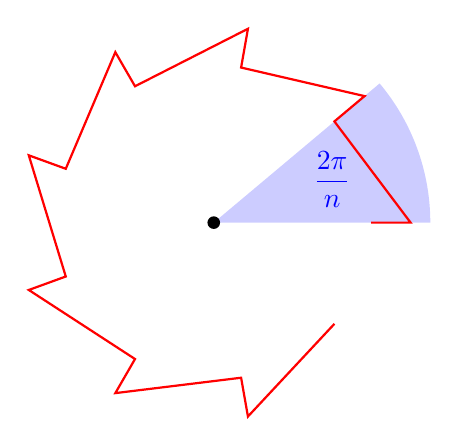
\begin{tikzpicture}[>=latex,thick]
\def\a{40}
\def\r{2}
\def\R{2.5}
\fill[color=blue!20] (0,0) -- (0:{1.1*\R}) arc (0:\a:{1.1*\R}) -- cycle;
\node[color=blue] at ({0.5*\a}:{0.8*\r}) {$\displaystyle\frac{2\pi}n$};
\fill (0,0) circle[radius=0.08];
\draw[color=red] (0:\r) -- (0:\R)
	-- ({1*\a}:\r) -- ({1*\a}:\R)
	-- ({2*\a}:\r) -- ({2*\a}:\R)
	-- ({3*\a}:\r) -- ({3*\a}:\R)
	-- ({4*\a}:\r) -- ({4*\a}:\R)
	-- ({5*\a}:\r) -- ({5*\a}:\R)
	-- ({6*\a}:\r) -- ({6*\a}:\R)
	-- ({7*\a}:\r) -- ({7*\a}:\R)
	-- ({8*\a}:\r) %-- ({8*\a}:\R)
;
\end{tikzpicture}
\end{center}
\[
C_n
=
\{\text{Drehungen um Winkel $2\pi/n$}\}
\]
\end{block}
\end{column}
\begin{column}{0.48\textwidth}
\begin{block}{Diedergruppen}
\begin{center}
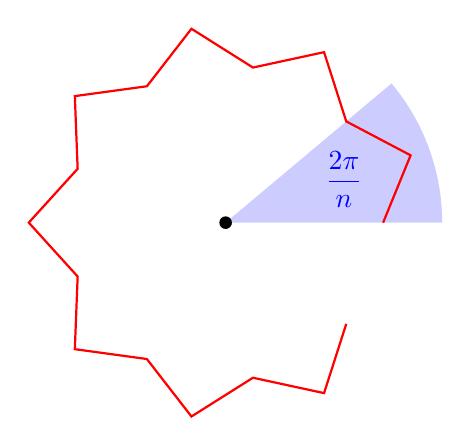
\begin{tikzpicture}[>=latex,thick]
\def\a{40}
\def\r{2}
\def\R{2.5}
\fill[color=blue!20] (0,0) -- (0:{1.1*\R}) arc (0:\a:{1.1*\R}) -- cycle;
\node[color=blue] at ({0.5*\a}:{0.8*\r}) {$\displaystyle\frac{2\pi}n$};
\fill (0,0) circle[radius=0.08];
\draw[color=red] (0:\r) -- ({0.5*\a}:\R)
	-- ({1*\a}:\r) -- ({1.5*\a}:\R)
	-- ({2*\a}:\r) -- ({2.5*\a}:\R)
	-- ({3*\a}:\r) -- ({3.5*\a}:\R)
	-- ({4*\a}:\r) -- ({4.5*\a}:\R)
	-- ({5*\a}:\r) -- ({5.5*\a}:\R)
	-- ({6*\a}:\r) -- ({6.5*\a}:\R)
	-- ({7*\a}:\r) -- ({7.5*\a}:\R)
	-- ({8*\a}:\r) %-- ({8.5*\a}:\R)
;
\end{tikzpicture}
\end{center}
\begin{align*}
D_n
&=
\langle\text{Spiegelung},
\text{Drehungen}\rangle
\\
&=
C_2
\ltimes
C_n
\end{align*}
\end{block}
\end{column}
\end{columns}
\end{frame}
\egroup
